\documentclass[11pt]{article}
\usepackage[margin=1in]{geometry}
\usepackage{amsmath,amssymb,amsthm,booktabs,graphicx,microtype}
\usepackage[numbers,sort&compress]{natbib}
\usepackage[hidelinks]{hyperref}
\graphicspath{{../results/figures/}}
\newcommand{\angstrom}{\ensuremath{\text{\normalfont\AA}}}
\newcommand{\pw}{\tau_{\mathrm{pw}}}
\newcommand{\Jung}{\sqrt{3/2}}
\newtheorem{theorem}{Theorem}
\newtheorem{lemma}{Lemma}
\newtheorem{proposition}{Proposition}
\title{Common Spatial Witnesses Reveal Higher-Order Geometry in Molecular Path Barcodes}
\author{}
\date{}

\begin{document}
\maketitle

\begin{abstract}
Three molecular interaction patches can intersect in pairs without sharing a spatial point. A path born from pairwise compatibility can therefore appear before its interactions are jointly realizable. Common-support persistent path homology (CS-PPH) assigns each path the first scale at which a single point satisfies every patch, with each patch allowing alternative atom contacts. The birth value comes with a numerical witness certificate, and an affine Jung bound controls its separation from the pairwise birth. Holding the graph and allowed paths fixed, the common-witness rule changes higher-order barcodes in RNA and protein--DNA structures while preserving connected-component persistence. The witness also has a direct spatial interpretation: with the annotated sites hidden, candidate witnesses cover 99.2\% of zinc sites and 94.5\% of structural-water sites within $2\,\angstrom$ in their respective structure cohorts. Common support connects a geometric question---where can these interactions hold together?---to both a persistent invariant and a coordinate that can be checked.
\end{abstract}

\section{Pairwise compatibility is not joint realizability}

Imagine three interaction patches, each admitting two of the same three locations. Each pair has a witness, but the three pairs use different locations. At that scale a pairwise rule fills the triangle, whereas the nerve of the actual supports leaves it hollow (Figure~\ref{fig:main}a). Pairwise compatibility answers whether each pair can work somewhere. It does not answer whether the interactions can all work in the same place.

This distinction matters when a chemically defined interaction can be realized by any of several atom contacts. Choosing one contact in advance discards valid alternatives; treating each pair independently can choose alternatives that cannot coexist. We represent every interaction as a union of admissible spatial supports and ask for one location shared by all the interactions on a path. Its first feasible scale is the birth of the path. The same calculation returns a point that can be checked against the selected atom contacts.

Common support brings the Čech--Rips distinction between joint and pairwise intersection to sets that need not be convex. Classical Čech--Rips comparisons control the two constructions for point sets\citep{chazal2014}; path homology gives a separate way to retain the ordering of interactions in a directed graph\citep{grigoryan2012,chowdhury2018}. We connect the two by using a support-set intersection to assign a birth to a chemically allowed path. The geometry sets the clock; the path complex sets the chains. This separation lets us change the birth rule without changing the molecular graph, and test whether that change reaches the barcode.

\begin{figure}[p]
\centering
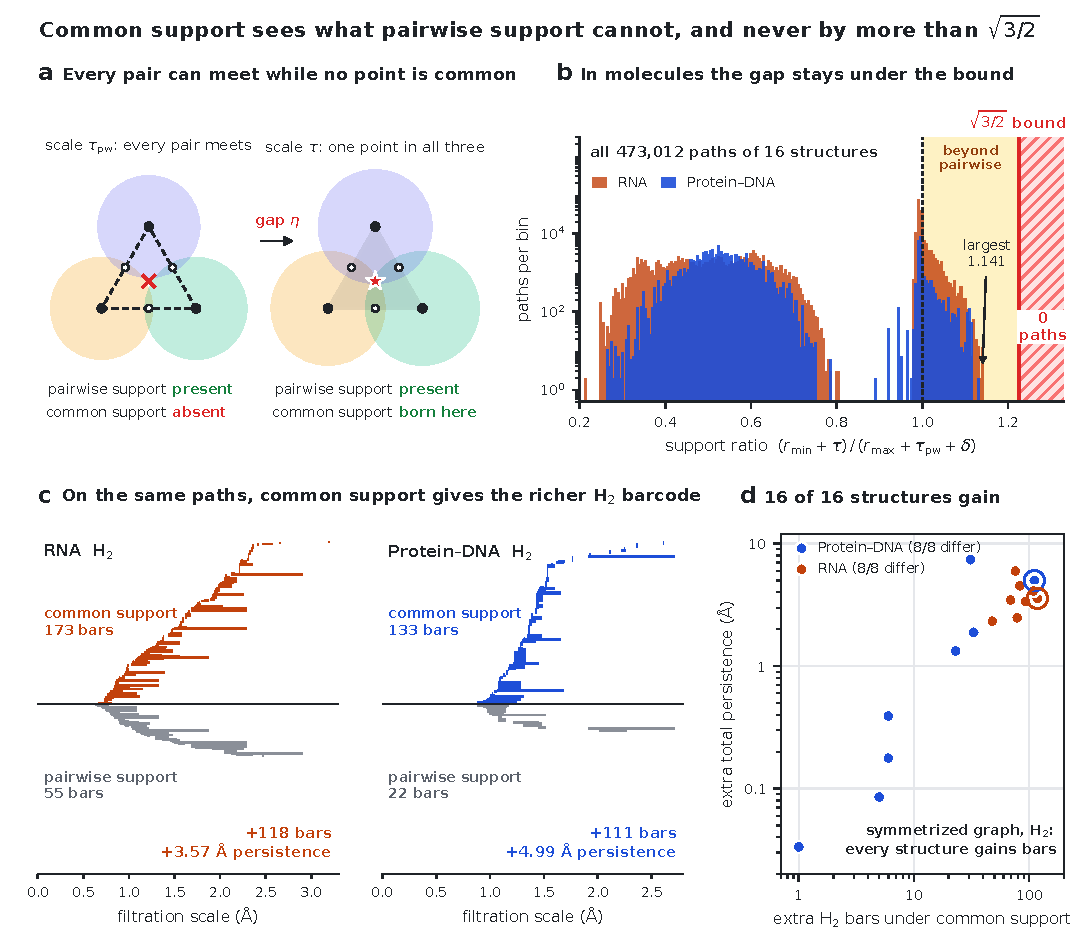
\includegraphics[width=\textwidth]{fig_common_support_main.pdf}
\caption{\textbf{A single witness distinguishes supports that pairwise intersections cannot.}
(a) Separate pairwise witnesses allow a filled triangle in the flag complex before the three supports share a point. This is a schematic of the support-set nerve and its flag completion, not a path-homology barcode.
(b) The audited paths obey the affine Jung bound on the normalized radius ratio $(r_{\min}+\tau)/(r_{\max}+\pw+\delta)$; a ratio above one certifies a positive support gap, but a positive gap can also occur below one.
(c) Example symmetrized $H_2$ barcodes use the same physical scale and allowed paths for both birth rules. (d) Each point is a structure; finite total persistence and interval count are separate readouts. Plotted and counted bars exceed the $0.01\,\angstrom$ minimum length. Total finite persistence sums finite lifetimes and does not include essential intervals.}
\label{fig:main}
\end{figure}

\section{A path birth has a checkable spatial witness}
\label{sec:definition}

\paragraph{From contacts to patch supports.}
Atom $v$ has position $x_v\in\mathbb R^3$, radius $r_v$ and closed ball $B_v(t)=\overline B(x_v,r_v+t)$ at scale $t\geq 0$. A directed microcontact $c=(a_c,b_c)$ connects a donor to an acceptor. Its support is the lens $L_c(t)=B_{a_c}(t)\cap B_{b_c}(t)$. A patch $P$ groups alternative microcontacts with the same donor and acceptor site identities, so its support is
\[
 S_P(t)=\bigcup_{c\in P}L_c(t).
\]
For the distinct patches $\mathcal P=\{P_1,\ldots,P_k\}$ on a path, define the common birth, the pairwise birth and their gap by
\begin{equation}
 \tau(\mathcal P)=\min\{t\geq 0:\bigcap_i S_{P_i}(t)\ne\varnothing\},
 \qquad
 \pw(\mathcal P)=\max_{\substack{\varnothing\ne J\subseteq[k]\\ |J|\leq 2}}\tau(\mathcal P_J),
 \qquad
 \eta=\tau-\pw.
 \label{eq:birth}
\end{equation}
The singleton convention gives the same vertex birth under both rules. These scales depend on the patch set; the order of the patches still matters to the path complex.

\paragraph{Choosing contacts and certifying a point.}
Write $V_\sigma$ for the endpoint atoms of a selection $\sigma$ of one microcontact per patch. For an atom set $V$, the weighted one-center value is
\[
 w(V)=\min_x\max\bigl\{0,\max_{v\in V}(\|x-x_v\|-r_v)\bigr\}.
\]
\begin{lemma}[Selection formula]
\label{lem:selection}
$\tau(\mathcal P)=\min_\sigma w(V_\sigma)$.
\end{lemma}
\begin{proof}
Distributing intersection over union gives $\bigcap_i S_{P_i}(t)=\bigcup_\sigma\bigcap_{v\in V_\sigma} B_v(t)$. The left side is nonempty exactly when a selection on the right is feasible.
\end{proof}

The solver searches the contact selections by branch and bound. Adding endpoint constraints cannot lower a support value, so a lower bound on a partial selection can rule out its entire branch. Each resolved selection yields a weighted one-center solution; the certificate checks the ball constraints and, at positive scale, checks optimality from active constraints. In three dimensions at most four active balls suffice for a fixed selection. The selected contacts and the point $x^*$ certify feasibility at the reported scale; the bounds on alternative selections establish minimality across selections. A local active-ball certificate does not by itself establish that global minimum. We distinguish failed or incomplete solves from a certified zero birth.

\begin{theorem}[Helly exactness and selection--Helly]
\label{thm:helly}
If every patch has one contact, the common birth equals the maximum birth over subfamilies of at most four patches. In general,
\begin{equation}
 \tau(\mathcal P)
   =\min_\sigma\max_{\substack{\varnothing\ne J\subseteq[k]\\ |J|\leq4}}w(V_{\sigma|J})
   \;\geq\;
     \max_{\substack{\varnothing\ne J\subseteq[k]\\ |J|\leq4}}\tau(\mathcal P_J).
 \label{eq:helly}
\end{equation}
\end{theorem}
\begin{proof}
For fixed $\sigma$, Helly's theorem in $\mathbb R^3$ reduces the common intersection of the endpoint balls to intersections of at most four balls\citep{helly1923}. Their endpoints belong to at most four selected contacts. This gives the inner maximum in~\eqref{eq:helly}; Lemma~\ref{lem:selection} gives the outer minimum. Exchanging the order of the maximum and minimum gives the lower bound. With one selection there is no exchange gap.
\end{proof}

\paragraph{Relation to Čech and Rips.}
The common birth is the Čech-type simplex birth in the nerve of the thickened patch supports. The pairwise birth is its Rips-type flag counterpart. With one zero-radius point per patch, the common birth is exactly the radius of the minimum enclosing ball of those points, recovering ordinary Čech. Two RNA point-cloud controls verify the reduction against an independent minimum enclosing ball and the persistence of an $\alpha$ complex (Table~\ref{tab:cech}). A patch with alternatives need not have convex support, so we do not invoke the good-cover nerve theorem or identify the barcode with the topology of the union of the supports.

\begin{table}[htbp]
\centering
\caption{\textbf{Single-point supports recover ordinary Čech.} The controls are RNA structures 1A9L and 1A60; they are separate from the molecular path cohort.}
\label{tab:cech}
\begin{tabular}{@{}lp{0.28\linewidth}@{}}
\toprule
Point-cloud control & Result \\
\midrule
Zero-radius common birth vs. independent minimum enclosing ball & Max. difference $1.1\times10^{-14}\,\angstrom$ \\
Čech vs. $\alpha$-complex interval endpoints & Max. difference $4.4\times10^{-16}\,\angstrom$ \\
Čech vs. point-cloud Rips & Different in $2/6$ structure--degree comparisons \\
\bottomrule
\end{tabular}
\end{table}

\section{The gap is real, and the radius ratio is bounded}
\label{sec:bound}

\paragraph{A shared point can appear strictly later.}
Place three sites at the vertices of an equilateral triangle of side $D$, with base radius $r<D/2$, and let patch $P_i$ support the other two sites. A pair of patches shares a site at scale zero. All three have no common point until two expanded balls first touch, at $D/2-r$. Thus $\pw=0$ but $\tau=D/2-r$ (Figure~\ref{fig:main}a). The same construction works with any finite number of sites: omit a different site from each patch and choose the sites at least $D$ apart, with one pair at distance exactly $D$. Every proper subfamily has a witness at scale zero, and the full family needs two sites' supports to meet. No fixed subfamily order determines general union-valued support. This construction concerns arbitrary patch families, not an observation of a gap beyond order four in the molecular cohort.

\paragraph{An affine Jung bound.}
Let $\delta_P$ be the largest distance between same-role endpoints of any two alternative contacts in patch $P$ (donor to donor or acceptor to acceptor). For a path let $\delta=\max_{P\in\mathcal P}\delta_P$ and let $r_{\min},r_{\max}$ be the extreme endpoint radii over its patches.

\begin{theorem}[Affine Jung bound]
\label{thm:jung}
The two birth rules satisfy
\begin{equation}
 \pw\leq\tau,
 \qquad
 r_{\min}+\tau\leq \Jung\,(r_{\max}+\pw+\delta).
 \label{eq:jung}
\end{equation}
For equal-radius single-contact patches the constant $\Jung$ is attained.
\end{theorem}
\begin{proof}
The lower bound follows by restricting any common witness to a pair. Fix a selection of one contact per patch. For each pair of patches a witness at $\pw$ lies within $r_{\max}+\pw$ of the endpoints of some qualifying pair of contacts. The corresponding endpoints of the fixed selection lie within an additional $\delta$ of these endpoints. Hence the selected centers have diameter at most $2(r_{\max}+\pw+\delta)$, including endpoints from the same patch by using a pair containing it. A singleton satisfies the bound directly. Jung's theorem in three dimensions places the selected centers inside a ball of radius at most $\Jung(r_{\max}+\pw+\delta)$\citep{jung1901}. Its center is in all selected endpoint balls at the resulting upper bound on $\tau$.

For sharpness, take four single-contact patches supported by equal-radius balls centered at the vertices of a regular tetrahedron of side $2r$ (a contact with coincident endpoint centers in this geometric example). The balls touch in pairs at $t=0$, but a common witness first exists at the tetrahedron's circumcenter, where $r+\tau=\Jung r$.
\end{proof}

Equation~\eqref{eq:jung} bounds a radius ratio, not $\tau/\pw$; the latter can be undefined even for a finite positive gap. Patch spread is essential to the general bound: moving the sites farther apart in the hollow-triangle construction increases $\tau$ while $\pw$ remains zero. Spread is not necessary for a gap, as the tetrahedron shows.

\paragraph{Molecular paths obey the bound, including the single-contact case.}
Figure~\ref{fig:main}b covers 340{,}874 RNA paths and 132{,}138 protein--DNA paths over both graph types and path orders zero through three. The maximum normalized ratios were 1.141 and 1.130, respectively, with no violations of~\eqref{eq:jung}. In protein--DNA, 9{,}616 paths composed entirely of single-contact patches had a positive gap at zero patch spread, across seven of eight structures, with a maximum gap of $0.676\,\angstrom$. In RNA, 43{,}078 of the 71{,}279 single-contact paths had a normalized ratio above one, certifying a positive gap. The molecular examples therefore distinguish joint from pairwise support even without patch alternatives. They do not test a strict gap beyond four-patch subfamilies.

\section{Changing the birth rule changes higher-order molecular barcodes}
\label{sec:barcodes}

\paragraph{The graph stays fixed.}
For either birth rule $\beta\in\{\tau,\pw\}$, let $A_t^\beta$ consist of the graph-allowed elementary paths with patch-set birth at most $t$. Births are monotone under taking subpaths. At each scale, the Grigor'yan--Lin--Muranov--Yau (GLMY) chain complex $\Omega_\bullet(A_t^\beta)$ retains the allowed chains whose boundaries are also allowed\citep{grigoryan2012,chowdhury2018}. Both rules act on the same final directed or symmetrized graph, with the same allowed paths, boundary and coefficient field.

\paragraph{The filtrations are interleaved, not identical.}
With graph-wide extrema $r_{\min},r_{\max},\delta$, set
\[
 \phi(t)=\max\{t,\Jung(r_{\max}+t+\delta)-r_{\min}\}.
\]
Theorem~\ref{thm:jung} gives $A_t^\tau\subseteq A_t^{\pw}\subseteq A_{\phi(t)}^\tau$. For $r_{\min}>0$, the change of variable $s=\log((r_{\min}+t)/r_{\min})$ bounds the shift by $\log(\Jung(r_{\max}+\delta)/r_{\min})$. The inclusions induce an interleaving of the path-homology modules and bound the bottleneck distance in that coordinate\citep{chazal2014,bauer2015}. The bound controls the possible disagreement; it neither requires equality nor measures the empirical bottleneck distance.

\paragraph{The difference reaches cycles and higher-dimensional classes.}
We compared the birth rules in eight RNA decoys and eight FTDMP bound protein--DNA decoys\citep{ftdmpdata}, each on a directed and a symmetrized graph. Within a structure and graph, we evaluated $H_0$--$H_2$ at the union of the actual path birth values in \angstrom, rather than at arbitrary grid points or by event index. An interval multiset can change through its endpoints even when its count stays fixed.

In both graph types, the RNA $H_1$ and $H_2$ barcodes differed in eight of eight structures. In protein--DNA, the directed graph differed in five of eight structures in $H_1$ and three of eight in $H_2$; five of eight differed in at least one degree. On symmetrized protein--DNA graphs, six of eight differed in $H_1$ and eight of eight in $H_2$. The $H_0$ barcodes agreed throughout: the rules coincide on the vertices and edges that govern connected-component persistence.

In symmetrized RNA $H_2$, the common rule added $2.33$--$5.96\,\angstrom$ of finite total persistence per structure. At the $0.01\,\angstrom$ minimum bar length, symmetrized $H_2$ gained 28--62 bars per RNA structure and 1--55 per protein--DNA structure (Figure~\ref{fig:main}c,d). Finite total persistence is the primary magnitude readout; counts describe the accompanying change and use that same minimum length throughout. The directed-graph companion figure is in the Supporting Information. In this fixed cohort, the most consistent differences occur beyond connected components, where the birth of a path can depend on more than two patches.

\section{The witness is a candidate coordinate for zinc and structural water}
\label{sec:sites}

Hiding a site turns joint realizability into a localization question: where can the surrounding ligand or polar-atom groups be satisfied at once? Each group supplies a union of atom-centered coordination supports. The same selection and one-center calculation supplies $x^*$ from the macromolecular atoms, without using the hidden coordinate to construct the candidate. We compare each annotated site with its closest candidate witness. Steric exclusion is a separate geometric filter on the resulting point rather than a change to the support optimization.

\begin{table}[htbp]
\centering
\caption{\textbf{Common witnesses localize hidden zinc and structural-water sites.} Each cohort contains 300 structures. Coverage is the fraction of annotated sites with at least one candidate witness within the stated radius; it is not one-to-one detection recall. Error is the median distance to the nearest witness. The certificate denominator counts weighted solves, not sites.}
\label{tab:sites}
\begin{tabular}{@{}lrrrrr@{}}
\toprule
Site type & Sites & $1\,\angstrom$ & $2\,\angstrom$ & Error (\angstrom) & Certificate failures \\
\midrule
Zinc & 640 & 90.2\% & 99.2\% & 0.142 & $0/157{,}715$ \\
Structural water & 9{,}441 & 57.9\% & 94.5\% & 0.852 & $0/14{,}824{,}091$ \\
\bottomrule
\end{tabular}
\end{table}

Pairwise feasibility and site coverage answer different questions. For candidate ligand groups, fix a coordination tolerance $t_{\mathrm{tol}}$. A pairwise-only hard negative satisfies $\pw\leq t_{\mathrm{tol}}<\tau$: every pair is feasible, yet no position satisfies the whole candidate at that tolerance. Among pairwise-passing zinc triplets, 51.9\% were hard negatives by this definition. The fraction was 26.8\% among the triplets retained after steric filtering and 8.6\% in the pairwise-passing classical-ligand stratum before that filter. These are candidate composition measurements, not classification accuracy. Together with Table~\ref{tab:sites}, they show what the witness contributes: a check on the joint configuration and a point for the configurations it supports.

\subsection{Time-separated external zinc comparison}
\label{sec:external}
% Reserved for Metal3D and AllMetal3D results on the common quality-controlled pool.
The external comparison pairs CS-PPH with Metal3D and AllMetal3D\citep{durr2023,durr2025} on the same quality-controlled zinc structures first released by the Protein Data Bank on or after 1 May 2024. This comparison uses one-to-one matching at $1$ and $2\,\angstrom$; it is distinct from the nearest-witness coverage in Table~\ref{tab:sites}. Comparative results are reserved for the matched evaluation.

\section{Discussion and conclusion}

The decisive change is the quantifier: a path no longer asks for a possibly different point for each pair, but one point for every interaction. That change gives the birth a spatial certificate. It preserves the close relationship between pairwise and common support expressed by the affine Jung bound while allowing their higher-order barcodes to differ. In the site examples the same object is immediately interpretable: the witness is a candidate position, not a scalar score translated into a location after the fact.

Geometry and prediction answer different questions. On fixed FTDMP bound candidate pairs that the physical-plus-pairwise model found ambiguous, adding barcode features improved ordering agreement beyond the support-summary features (Supporting Information). This is a targeted feature ablation: it tests whether the barcode representation adds information in otherwise difficult comparisons, not whether a ranked list is better on every candidate pool. Same-pool external scoring is reported as context in the Supporting Information.

Common support extends a familiar idea from point-cloud topology to directed paths with alternative molecular contacts. It identifies joint interactions that a pairwise rule cannot recover, gives their scale a checkable geometric meaning, and carries the distinction into persistence without changing the underlying graph.

\section*{Data and code availability}
The \href{https://github.com/Neabigmo/GSPH}{CS-PPH repository} provides the mathematical specification, evidence register, cohort manifests, scripts, and consolidated results. The FTDMP candidate structures are distributed separately by their authors\citep{ftdmpdata}.

\section*{Supporting Information}
Solver certificates and stability; event-based path persistence and directed-graph results; site-localization metrics; frozen hard-pair ablation; same-pool external scoring.

\bibliographystyle{unsrtnat}
\bibliography{refs}
\end{document}
